\documentclass[a4paper,12pt]{article}
\usepackage[utf8]{vietnam}
\usepackage{hyperref}
\usepackage{graphicx}
\usepackage{xcolor}
\usepackage{subfigure}
\usepackage{float}
\usepackage{caption}
\hypersetup{
	pdfborder = {0 0 0}
}
\title{\textbf{Báo cáo tuần 5 \\ Thực hành kiến trúc máy tính}}
\author{Họ tên: Phan Minh Anh Tuấn \\ MSSV: 20205227}
\date{}
\begin{document}
	\maketitle
	\tableofcontents
	\newpage
\section{Assignment 1}
\begin{figure}[!h]
	\centerline{\fbox{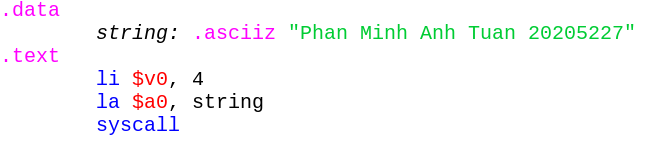
\includegraphics[width=0.7\textwidth]{ass1/code.png}}}
	\caption{Code của Assignment 1}
	\label{fig:ass1}
\end{figure}
\noindent
\textbf{Giải thích: }Phần dữ liệu đầu vào được thể hiện ở 2 dòng đầu. Phần thực thi, để in ra màn hình, cần gán thanh ghi \$v0 giá trị 4 (print string) sau đó load địa chỉ string vào \$a0. Kết quả của đoạn code được thể hiện tại Hình \ref{fig:ass1_result}
\begin{figure}[!h]
	\centerline{\fbox{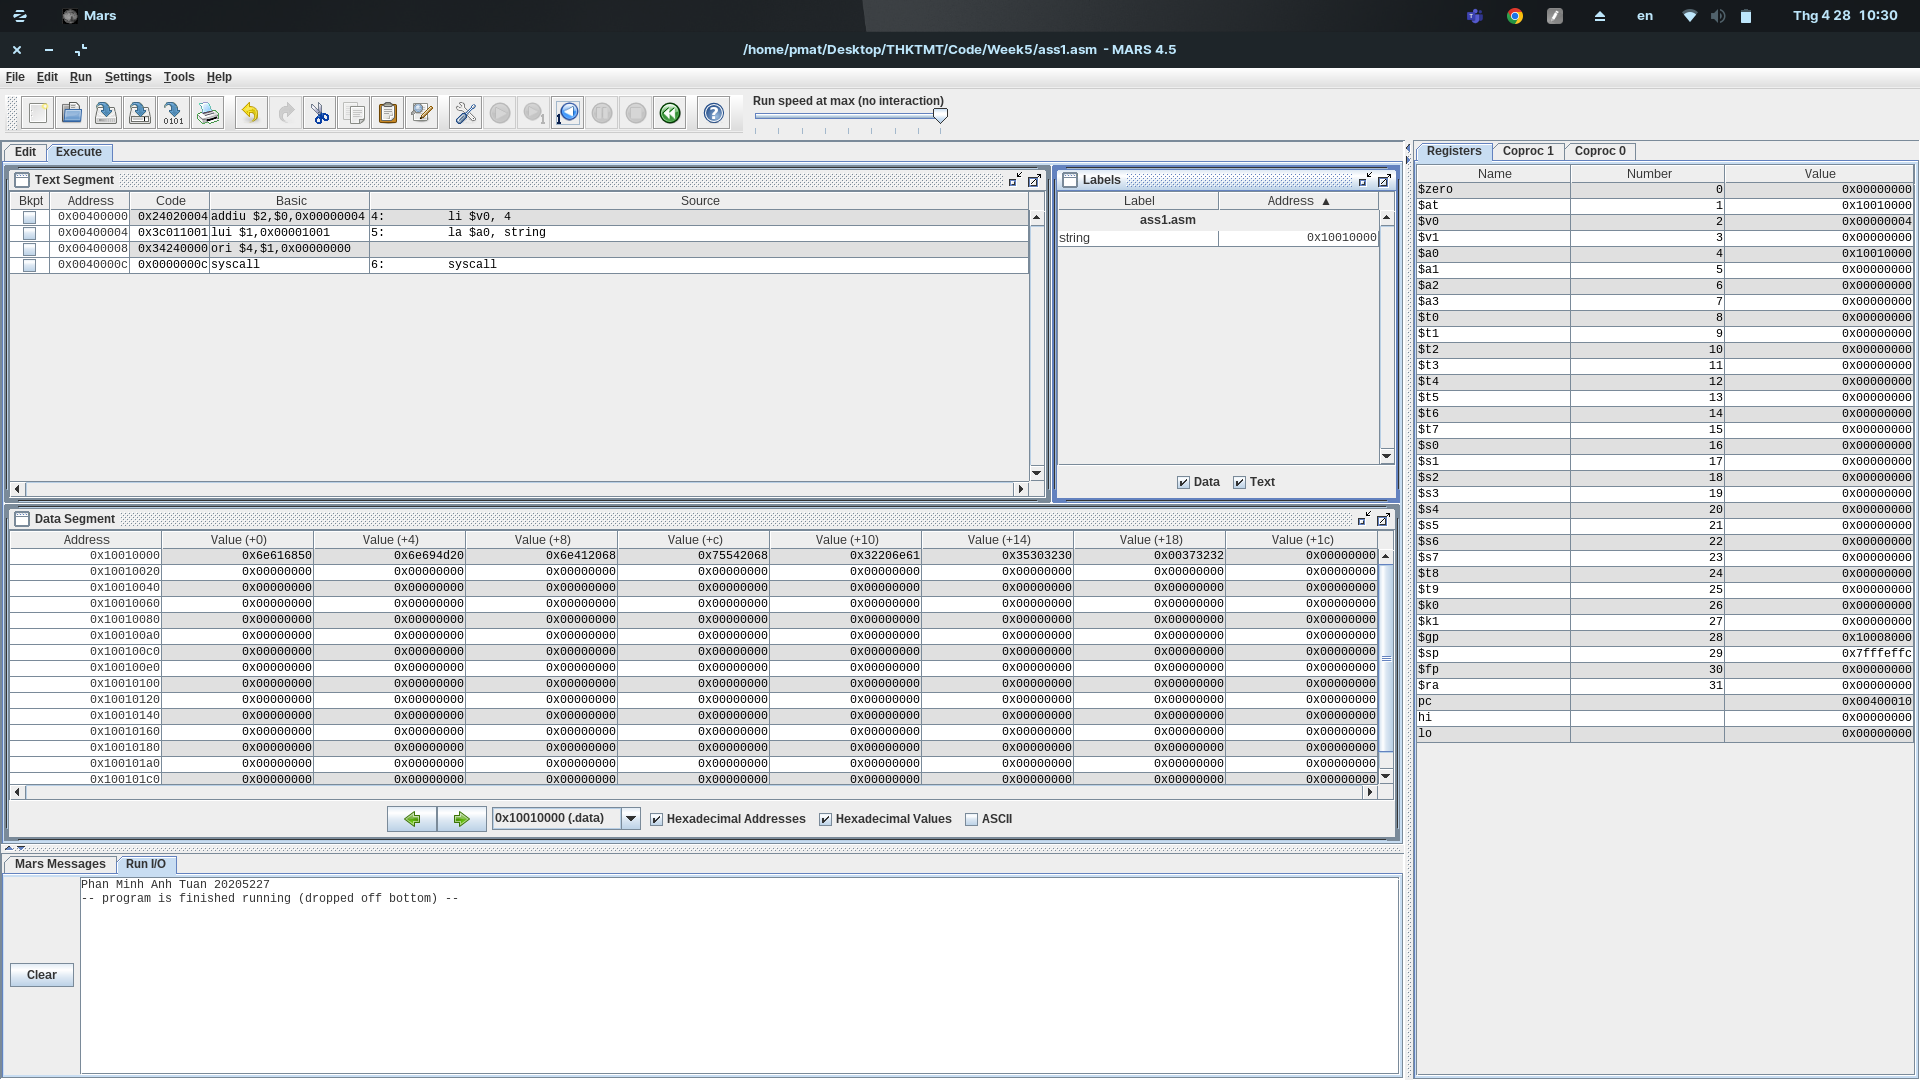
\includegraphics[width=0.9\textwidth]{ass1/result.png}}}
	\caption{Kết quả của Assignment 1}
	\label{fig:ass1_result}
\end{figure}	
\clearpage
\section{Assignment 2}
\begin{figure}[!h]
	\centerline{\fbox{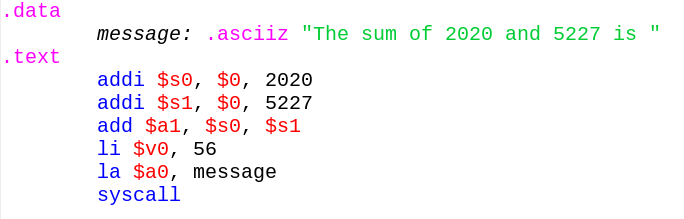
\includegraphics[width=0.7\textwidth]{ass2/code.png}}}
	\caption{Code của Assignment 2}
	\label{fig:ass2}
\end{figure}
\noindent
\textbf{Giải thích: }Thực hiện gán giá trị \$s0 và \$s1 sau đó tính tổng và gán vào \$a1. Để in ra màn hình, cần gán thanh ghi \$v0 giá trị 56 (MessageDialogInt). Kết quả của đoạn code được thể hiện tại Hình \ref{fig:ass1_result}
\begin{figure}[!h]
	\centerline{\fbox{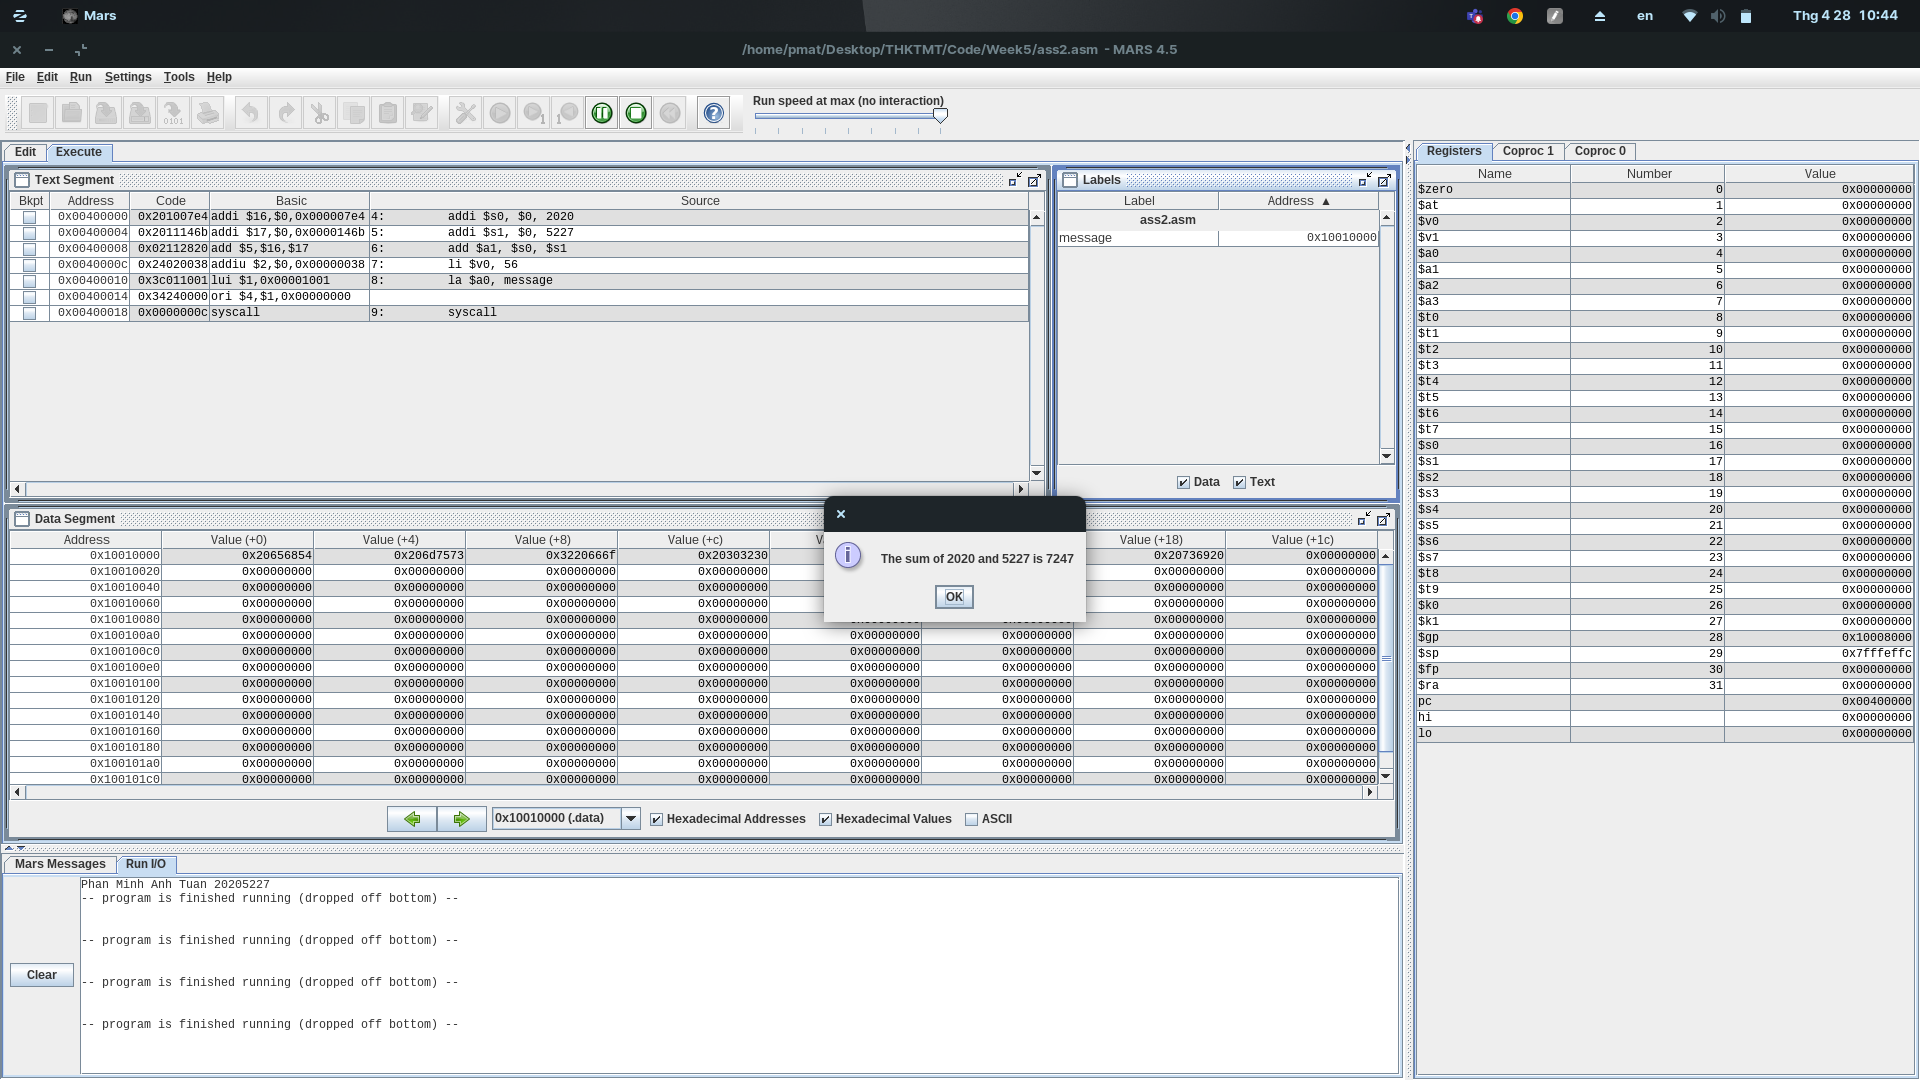
\includegraphics[width=0.9\textwidth]{ass2/result.png}}}
	\caption{Kết quả của Assignment 2}
	\label{fig:ass2_result}
\end{figure}	
\clearpage
\section{Assignment 3}
\begin{figure}[!h]
	\centerline{\fbox{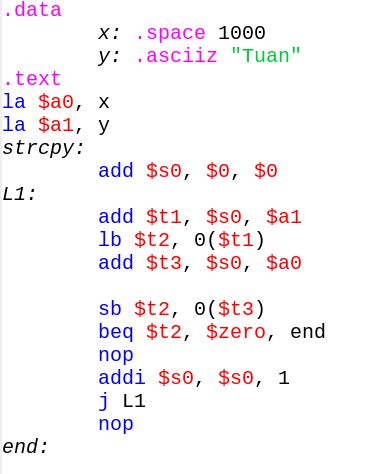
\includegraphics[width=0.7\textwidth]{ass3/code.png}}}
	\caption{Code của Assignment 3}
	\label{fig:ass3}
\end{figure}
\noindent
\textbf{Trong đó: }
\begin{itemize}
	\item x là xâu được copy ra
	\item y là xâu gốc
	\item \$s0 là current của xâu, bắt đầu từ 0
	\item \$t1 là địa chỉ của xâu gốc tại current \$s0
	\item \$t2 là giá trị tại địa chỉ \$t1
	\item \$t3 là địa chỉ của xâu được copy tại current \$s0
\end{itemize}
\newpage
\noindent
\textbf{Giải thích: }Chương trình thực hiện copy từng phần tử 1 từ xâu y sang xâu x. Với mỗi bước lặp mình gán giá trị \$t2 vào giá trị tại địa chỉ \$t3, cho đến khi \$t2 bằng 0 thì dừng lại.
\begin{figure}[!h]
	\centerline{\fbox{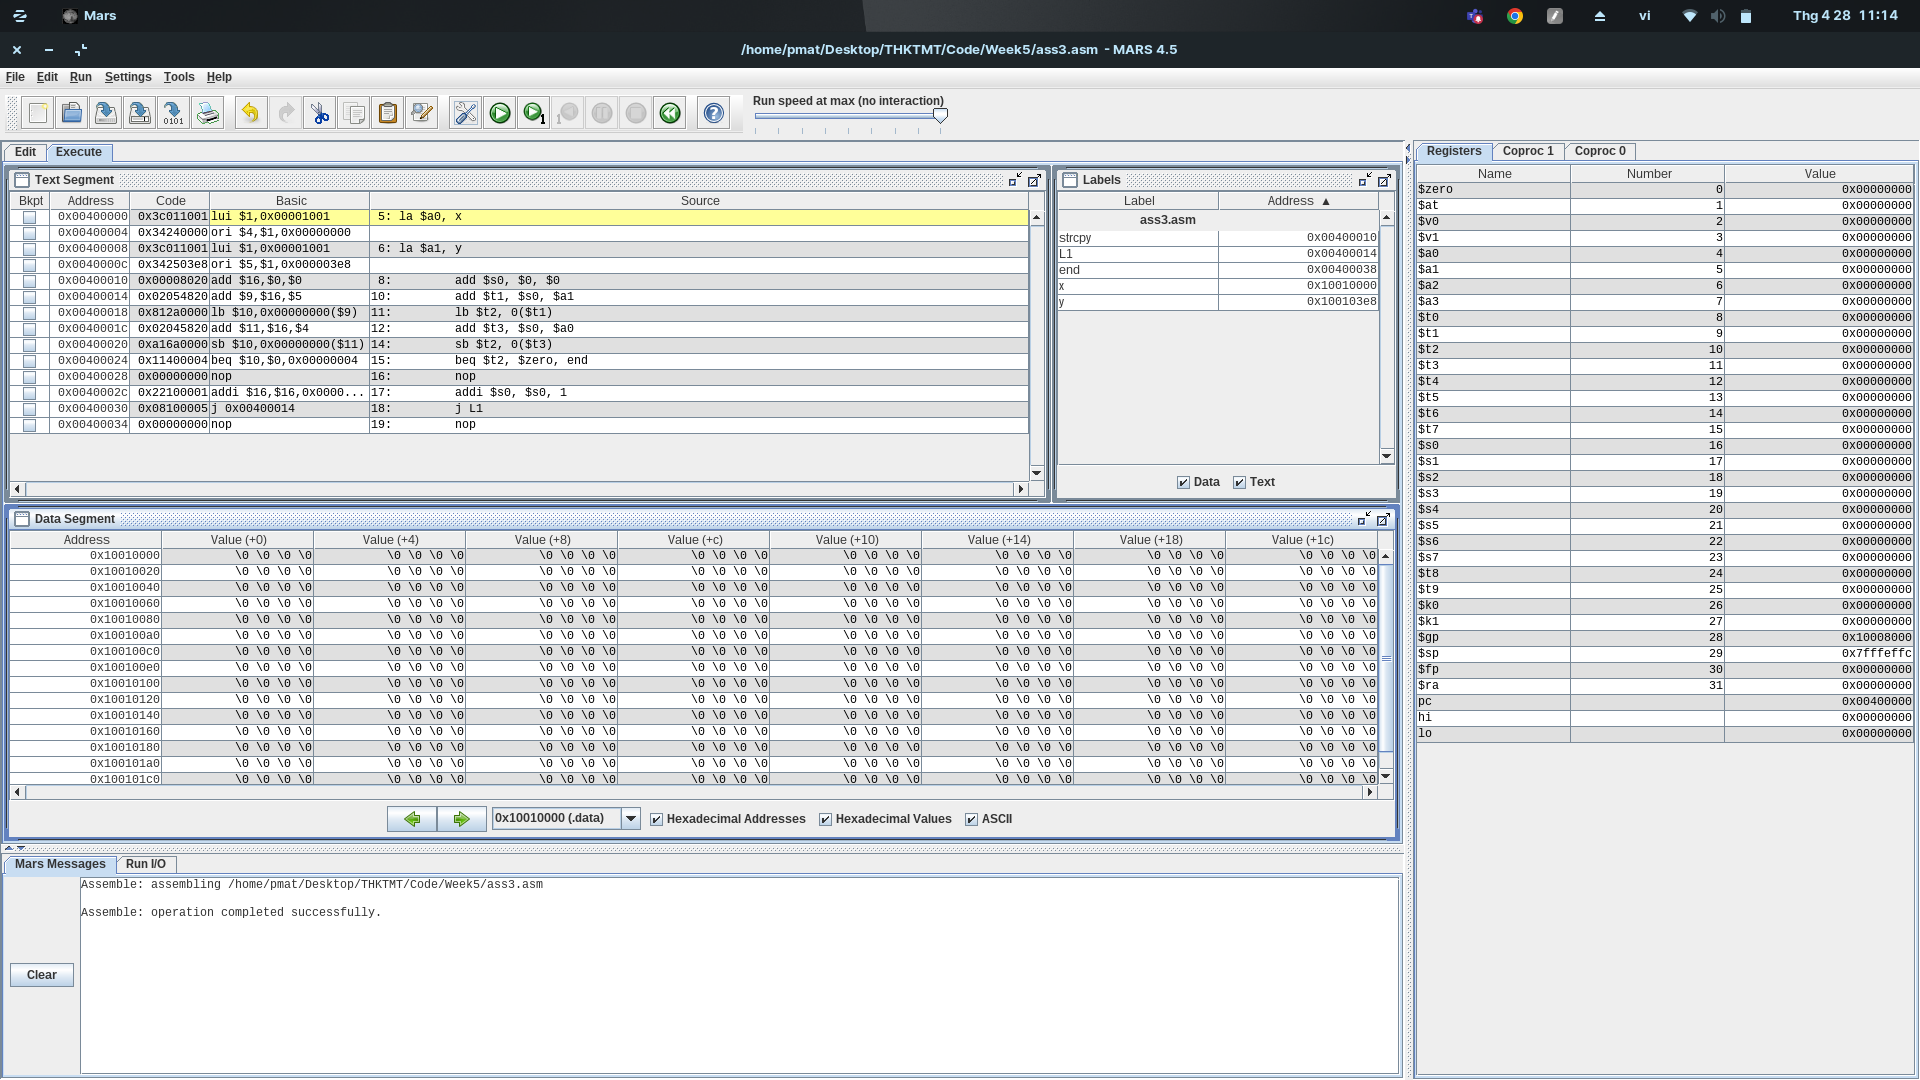
\includegraphics[width=0.9\textwidth]{ass3/result1.png}}}
	\caption{Kết quả trước khi chạy}
	\label{fig:ass3_r1}
\end{figure}
\begin{figure}[!h]
	\centerline{\fbox{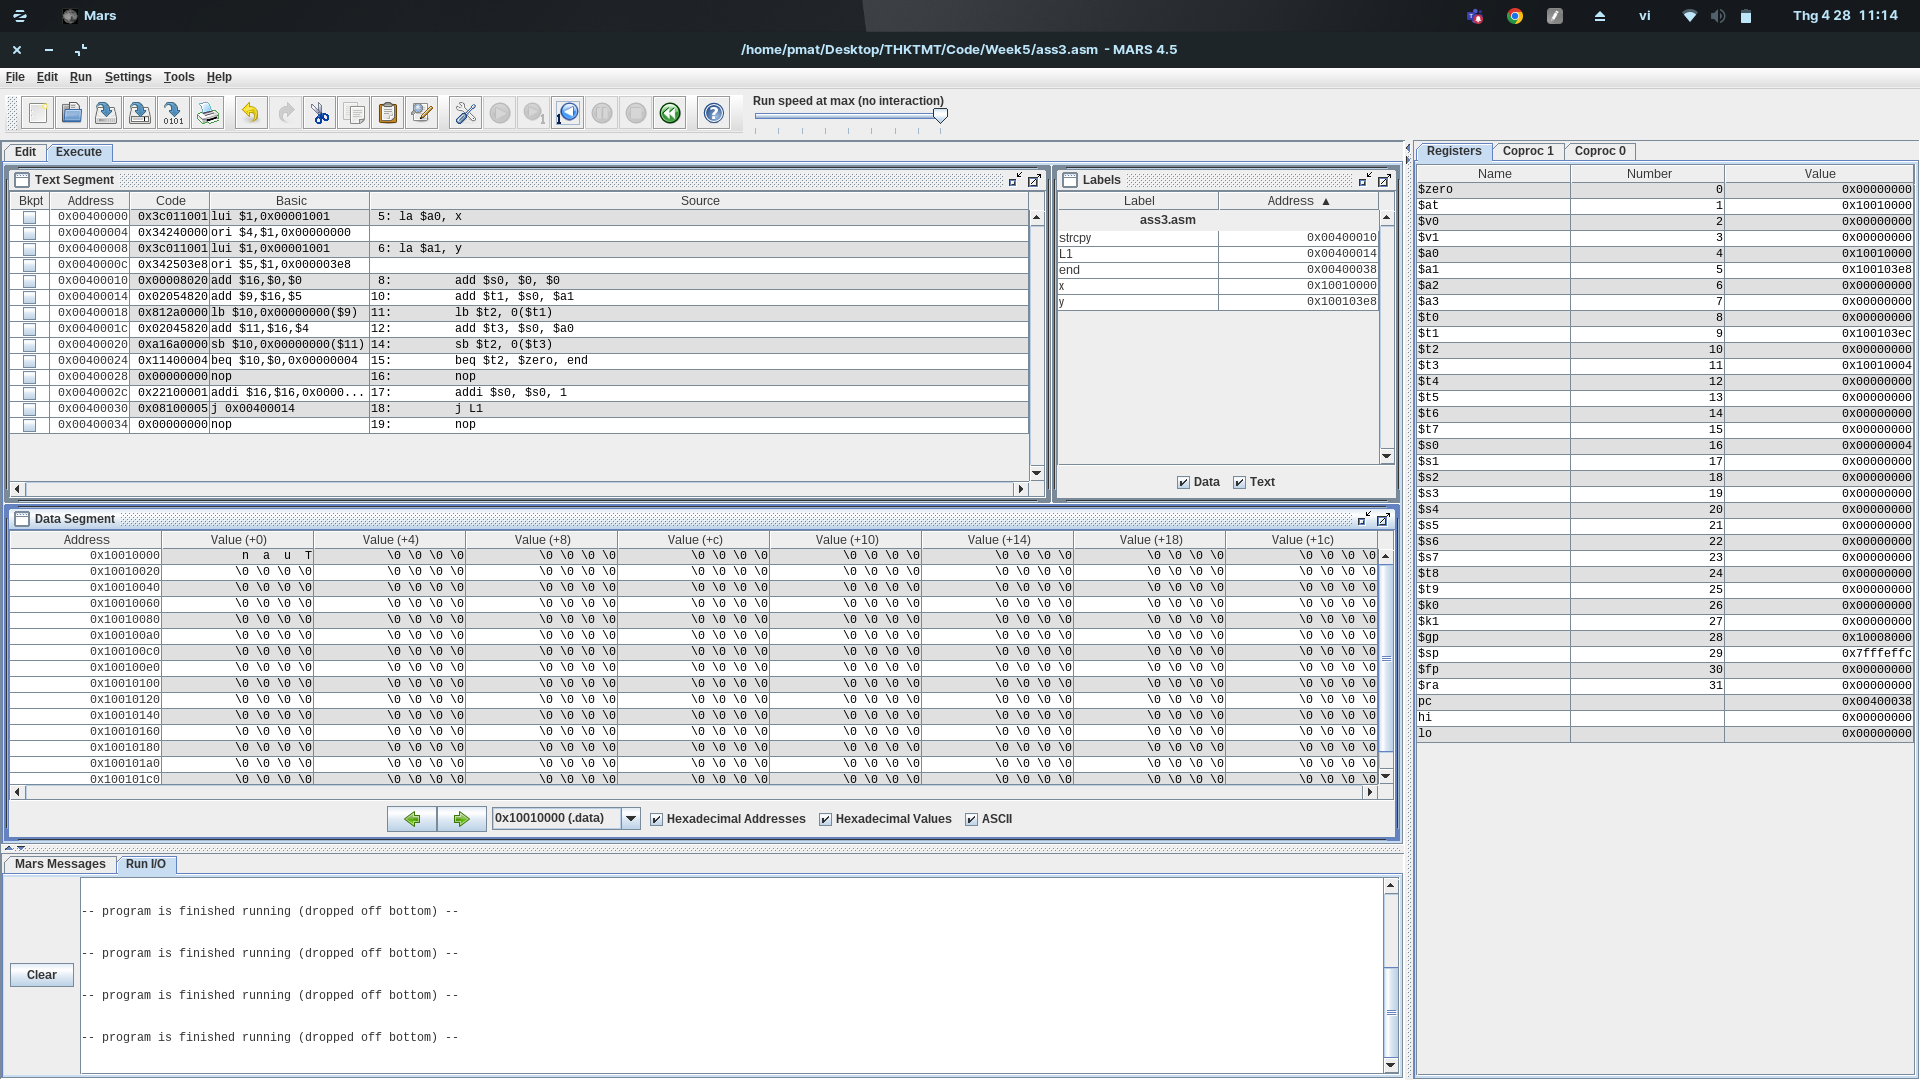
\includegraphics[width=0.9\textwidth]{ass3/result2.png}}}
	\caption{Kết quả sau khi chạy}
	\label{fig:ass3_r2}
\end{figure}
\clearpage
\section{Assignment 4}
\begin{figure}[!h]
	\centerline{\fbox{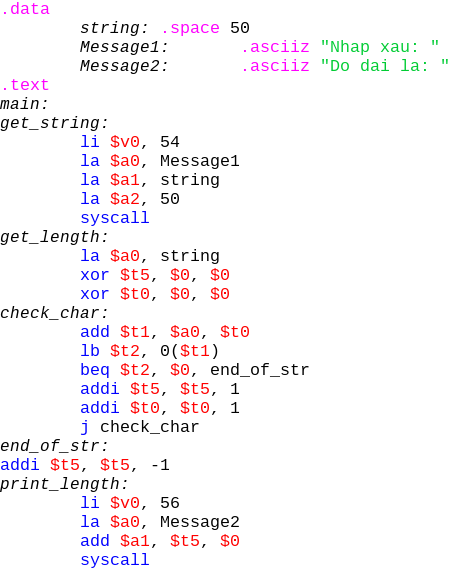
\includegraphics[width=0.6\textwidth]{ass4/code.png}}}
	\caption{Code của Assignment 4}
	\label{fig:ass4}
\end{figure}
\noindent
\textbf{Trong đó: }
\begin{itemize}
	\item string: Chuỗi nhập vào từ bàn phím
	\item Message1: Thông báo thứ 1
	\item Message2: Thông báo thứ 2
	\item get\_string: Phần xử lý nhập vào từ bàn phím
	\item get\_length: Đếm độ dài của xâu
	\item check\_char: Kiểm tra xem đó có phải kí tự hợp lệ không, nếu không thoát khỏi vòng lặp
	\item print\_length: In ra số phần tử của xâu
\end{itemize}
\newpage
\noindent
\textbf{Giải thích: }
\begin{itemize}
	\item get\_string: Nhập xâu vào từ bàn phím, sử dụng \$v0 = 54 (InputDialogString). Xâu được nhập vào lưu trữ tại string.
	\item get\_length: Lấy địa chỉ của xâu string lưu vào thanh ghi \$a0. \$t5 là thanh ghi lưu trữ độ dài của xâu, \$t0 là offset.
	\item check\_char: \$t1 là địa chỉ của kí tự vị trí \$t0 của xâu string. \$t2 là giá trị của địa chỉ \$t1. Nếu \$t2 là null, kết thúc vòng lặp. Nếu không, thực hiện tăng bộ đếm và độ dài của xâu và tiếp tục vòng lặp.
	\item print\_length: In ra số phần tử của xâu qua \$v0 (MessageDialogInt)
\end{itemize}
\begin{figure}[!h]
	\centerline{\fbox{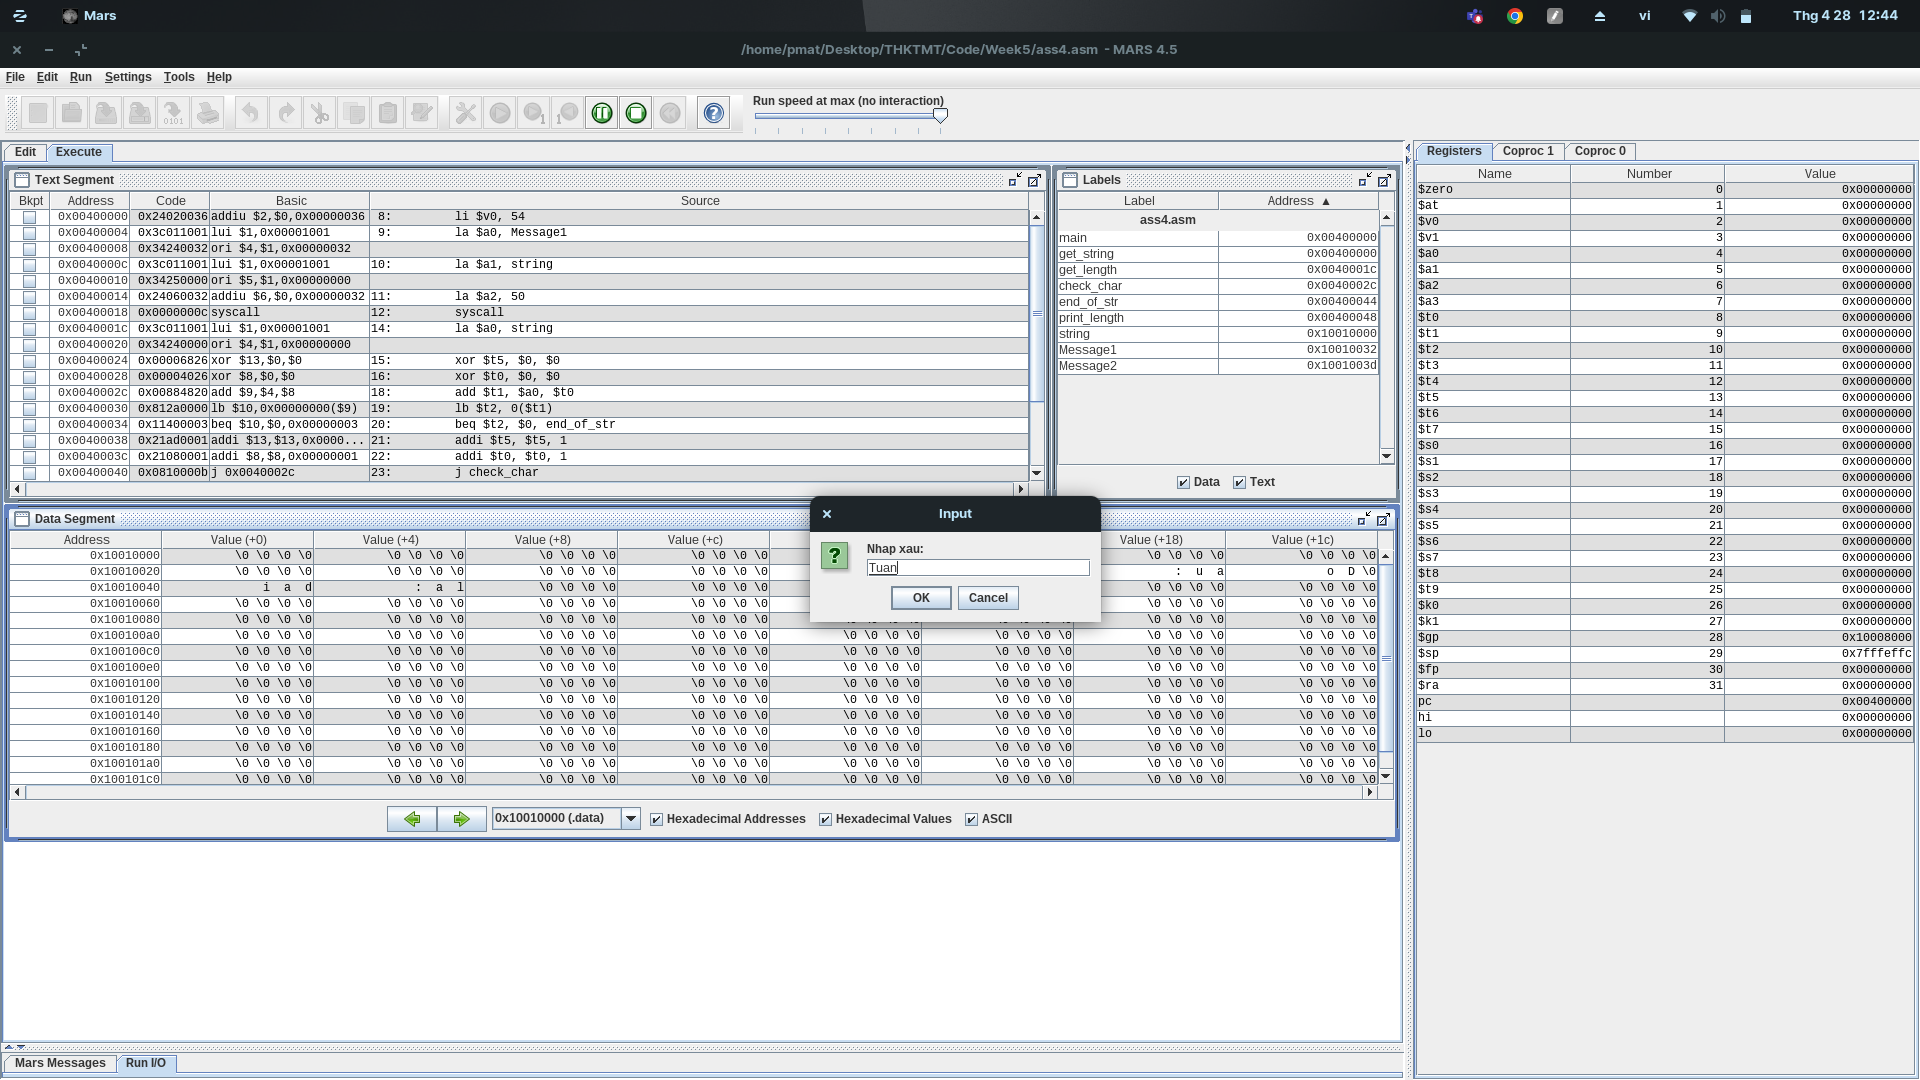
\includegraphics[width=0.55\textwidth]{ass4/result1.png}}}
	\caption{Kết quả trước khi chạy}
	\label{fig:ass4_r1}
\end{figure}
\begin{figure}[!h]
	\centerline{\fbox{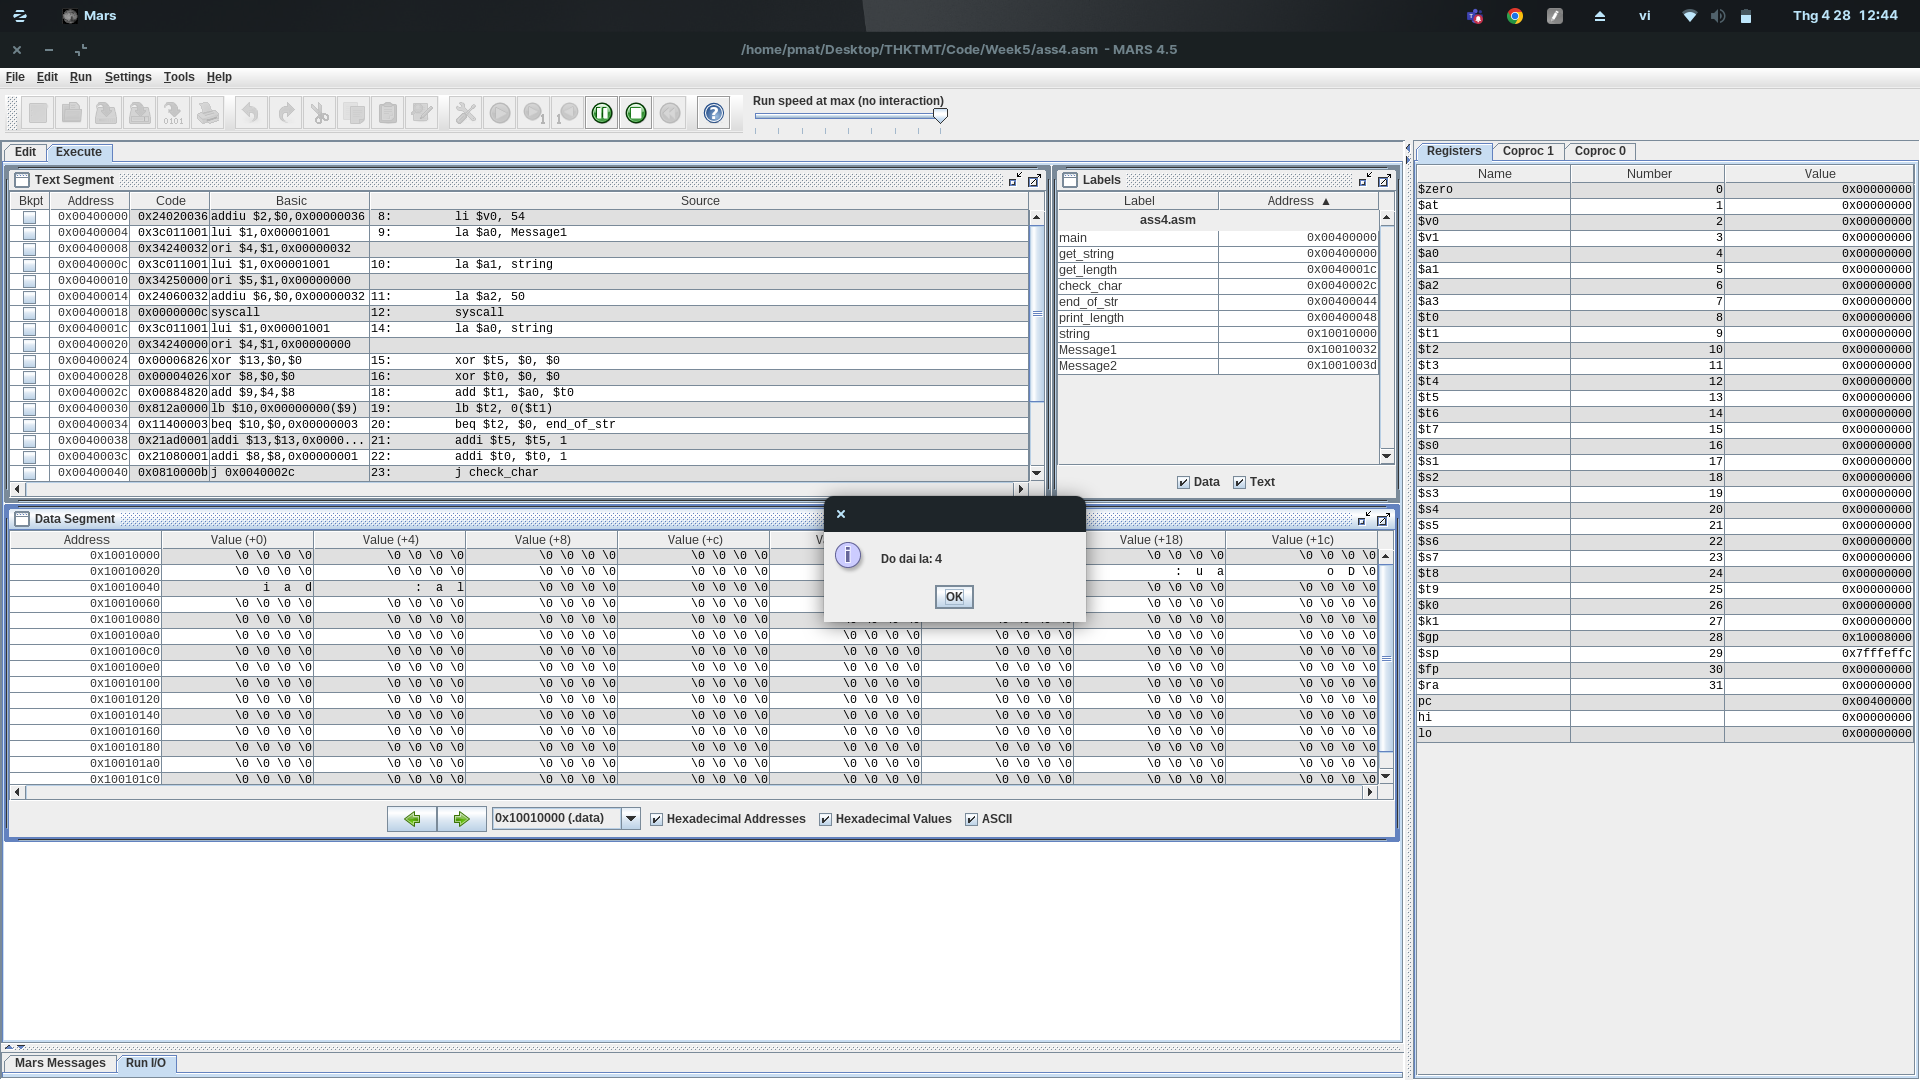
\includegraphics[width=0.55\textwidth]{ass4/result2.png}}}
	\caption{Kết quả sau khi chạy}
	\label{fig:ass4_r2}
\end{figure}
\clearpage
\section{Assignment 5}
\begin{figure}[!h]
	\centerline{\fbox{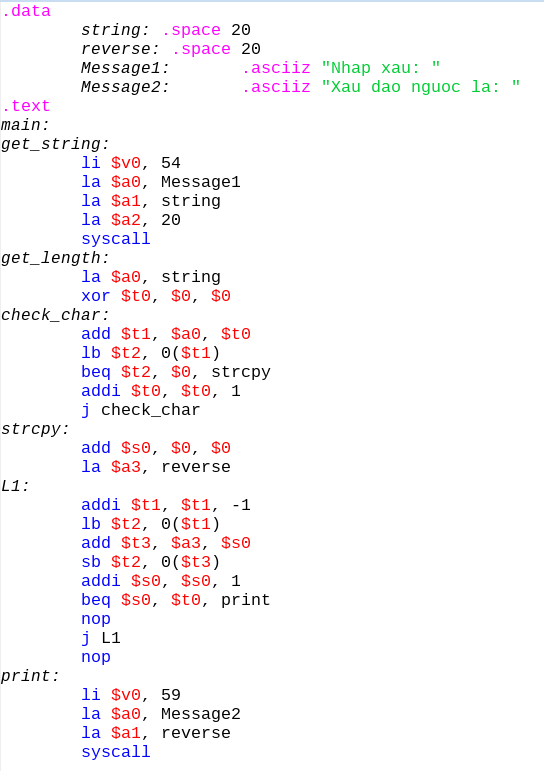
\includegraphics[width=0.6\textwidth]{ass5/code.png}}}
	\caption{Code của Assignment 5}
	\label{fig:ass5}
\end{figure}
\noindent
\textbf{Giải thích: }ta đếm số lượng phần tử (Assignment 4), sau đó strcpy (Assignment 3) từ cuối lên đầu. Đặt giới hạn cả string (input) và reverse(output) là 20. 
\begin{figure}[!h]
	\centerline{\fbox{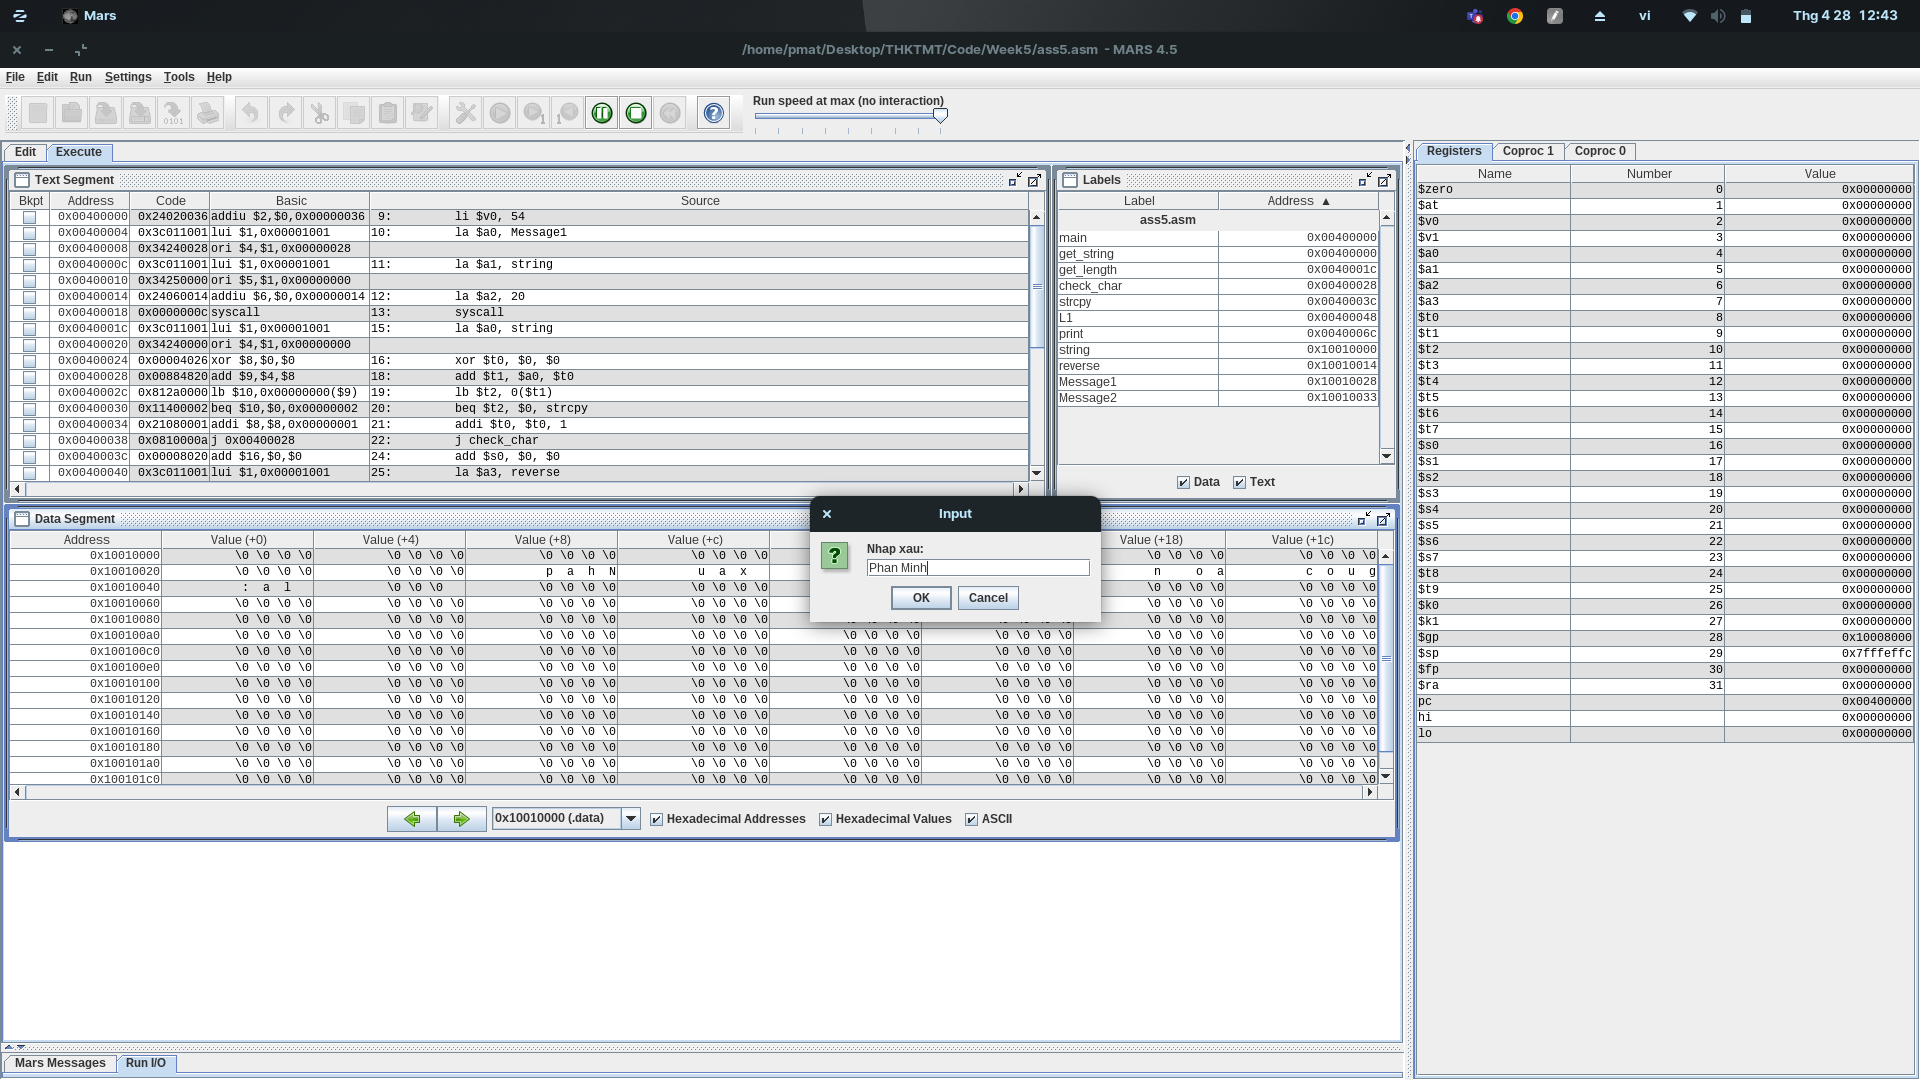
\includegraphics[width=0.9\textwidth]{ass5/result1.png}}}
	\caption{Kết quả trước khi chạy}
	\label{fig:ass5_r1}
\end{figure}
\begin{figure}[!h]
	\centerline{\fbox{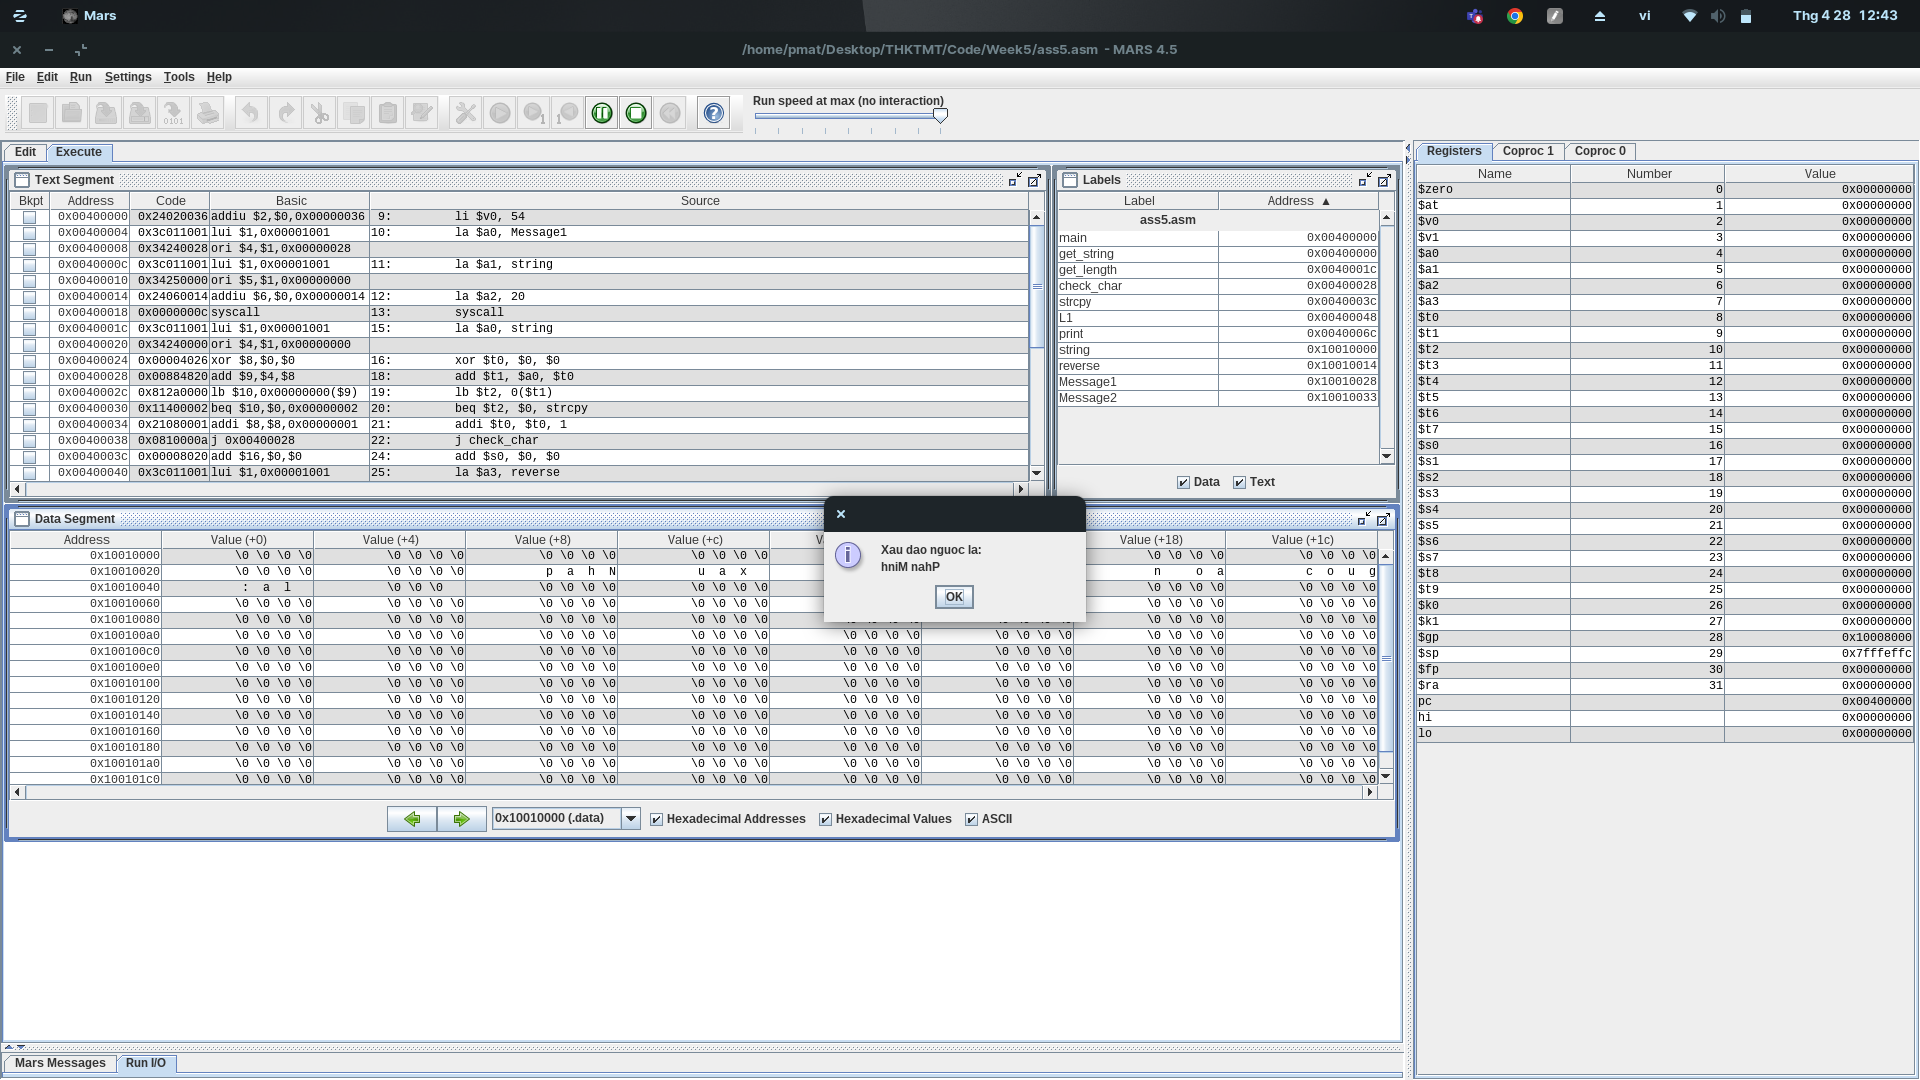
\includegraphics[width=0.9\textwidth]{ass5/result2.png}}}
	\caption{Kết quả sau khi chạy}
	\label{fig:ass5_r2}
\end{figure}
\end{document}